% Options for packages loaded elsewhere
\PassOptionsToPackage{unicode}{hyperref}
\PassOptionsToPackage{hyphens}{url}
%
\documentclass[
]{article}
\usepackage{amsmath,amssymb}
\usepackage{iftex}
\ifPDFTeX
  \usepackage[T1]{fontenc}
  \usepackage[utf8]{inputenc}
  \usepackage{textcomp} % provide euro and other symbols
\else % if luatex or xetex
  \usepackage{unicode-math} % this also loads fontspec
  \defaultfontfeatures{Scale=MatchLowercase}
  \defaultfontfeatures[\rmfamily]{Ligatures=TeX,Scale=1}
\fi
\usepackage{lmodern}
\ifPDFTeX\else
  % xetex/luatex font selection
\fi
% Use upquote if available, for straight quotes in verbatim environments
\IfFileExists{upquote.sty}{\usepackage{upquote}}{}
\IfFileExists{microtype.sty}{% use microtype if available
  \usepackage[]{microtype}
  \UseMicrotypeSet[protrusion]{basicmath} % disable protrusion for tt fonts
}{}
\makeatletter
\@ifundefined{KOMAClassName}{% if non-KOMA class
  \IfFileExists{parskip.sty}{%
    \usepackage{parskip}
  }{% else
    \setlength{\parindent}{0pt}
    \setlength{\parskip}{6pt plus 2pt minus 1pt}}
}{% if KOMA class
  \KOMAoptions{parskip=half}}
\makeatother
\usepackage{xcolor}
\usepackage[margin=1in]{geometry}
\usepackage{color}
\usepackage{fancyvrb}
\newcommand{\VerbBar}{|}
\newcommand{\VERB}{\Verb[commandchars=\\\{\}]}
\DefineVerbatimEnvironment{Highlighting}{Verbatim}{commandchars=\\\{\}}
% Add ',fontsize=\small' for more characters per line
\usepackage{framed}
\definecolor{shadecolor}{RGB}{248,248,248}
\newenvironment{Shaded}{\begin{snugshade}}{\end{snugshade}}
\newcommand{\AlertTok}[1]{\textcolor[rgb]{0.94,0.16,0.16}{#1}}
\newcommand{\AnnotationTok}[1]{\textcolor[rgb]{0.56,0.35,0.01}{\textbf{\textit{#1}}}}
\newcommand{\AttributeTok}[1]{\textcolor[rgb]{0.13,0.29,0.53}{#1}}
\newcommand{\BaseNTok}[1]{\textcolor[rgb]{0.00,0.00,0.81}{#1}}
\newcommand{\BuiltInTok}[1]{#1}
\newcommand{\CharTok}[1]{\textcolor[rgb]{0.31,0.60,0.02}{#1}}
\newcommand{\CommentTok}[1]{\textcolor[rgb]{0.56,0.35,0.01}{\textit{#1}}}
\newcommand{\CommentVarTok}[1]{\textcolor[rgb]{0.56,0.35,0.01}{\textbf{\textit{#1}}}}
\newcommand{\ConstantTok}[1]{\textcolor[rgb]{0.56,0.35,0.01}{#1}}
\newcommand{\ControlFlowTok}[1]{\textcolor[rgb]{0.13,0.29,0.53}{\textbf{#1}}}
\newcommand{\DataTypeTok}[1]{\textcolor[rgb]{0.13,0.29,0.53}{#1}}
\newcommand{\DecValTok}[1]{\textcolor[rgb]{0.00,0.00,0.81}{#1}}
\newcommand{\DocumentationTok}[1]{\textcolor[rgb]{0.56,0.35,0.01}{\textbf{\textit{#1}}}}
\newcommand{\ErrorTok}[1]{\textcolor[rgb]{0.64,0.00,0.00}{\textbf{#1}}}
\newcommand{\ExtensionTok}[1]{#1}
\newcommand{\FloatTok}[1]{\textcolor[rgb]{0.00,0.00,0.81}{#1}}
\newcommand{\FunctionTok}[1]{\textcolor[rgb]{0.13,0.29,0.53}{\textbf{#1}}}
\newcommand{\ImportTok}[1]{#1}
\newcommand{\InformationTok}[1]{\textcolor[rgb]{0.56,0.35,0.01}{\textbf{\textit{#1}}}}
\newcommand{\KeywordTok}[1]{\textcolor[rgb]{0.13,0.29,0.53}{\textbf{#1}}}
\newcommand{\NormalTok}[1]{#1}
\newcommand{\OperatorTok}[1]{\textcolor[rgb]{0.81,0.36,0.00}{\textbf{#1}}}
\newcommand{\OtherTok}[1]{\textcolor[rgb]{0.56,0.35,0.01}{#1}}
\newcommand{\PreprocessorTok}[1]{\textcolor[rgb]{0.56,0.35,0.01}{\textit{#1}}}
\newcommand{\RegionMarkerTok}[1]{#1}
\newcommand{\SpecialCharTok}[1]{\textcolor[rgb]{0.81,0.36,0.00}{\textbf{#1}}}
\newcommand{\SpecialStringTok}[1]{\textcolor[rgb]{0.31,0.60,0.02}{#1}}
\newcommand{\StringTok}[1]{\textcolor[rgb]{0.31,0.60,0.02}{#1}}
\newcommand{\VariableTok}[1]{\textcolor[rgb]{0.00,0.00,0.00}{#1}}
\newcommand{\VerbatimStringTok}[1]{\textcolor[rgb]{0.31,0.60,0.02}{#1}}
\newcommand{\WarningTok}[1]{\textcolor[rgb]{0.56,0.35,0.01}{\textbf{\textit{#1}}}}
\usepackage{longtable,booktabs,array}
\usepackage{calc} % for calculating minipage widths
% Correct order of tables after \paragraph or \subparagraph
\usepackage{etoolbox}
\makeatletter
\patchcmd\longtable{\par}{\if@noskipsec\mbox{}\fi\par}{}{}
\makeatother
% Allow footnotes in longtable head/foot
\IfFileExists{footnotehyper.sty}{\usepackage{footnotehyper}}{\usepackage{footnote}}
\makesavenoteenv{longtable}
\usepackage{graphicx}
\makeatletter
\newsavebox\pandoc@box
\newcommand*\pandocbounded[1]{% scales image to fit in text height/width
  \sbox\pandoc@box{#1}%
  \Gscale@div\@tempa{\textheight}{\dimexpr\ht\pandoc@box+\dp\pandoc@box\relax}%
  \Gscale@div\@tempb{\linewidth}{\wd\pandoc@box}%
  \ifdim\@tempb\p@<\@tempa\p@\let\@tempa\@tempb\fi% select the smaller of both
  \ifdim\@tempa\p@<\p@\scalebox{\@tempa}{\usebox\pandoc@box}%
  \else\usebox{\pandoc@box}%
  \fi%
}
% Set default figure placement to htbp
\def\fps@figure{htbp}
\makeatother
\setlength{\emergencystretch}{3em} % prevent overfull lines
\providecommand{\tightlist}{%
  \setlength{\itemsep}{0pt}\setlength{\parskip}{0pt}}
\setcounter{secnumdepth}{-\maxdimen} % remove section numbering
\usepackage{bookmark}
\IfFileExists{xurl.sty}{\usepackage{xurl}}{} % add URL line breaks if available
\urlstyle{same}
\hypersetup{
  hidelinks,
  pdfcreator={LaTeX via pandoc}}

\author{}
\date{\vspace{-2.5em}}

\begin{document}

\section{Mapping prescribed fires from a point and a date: a pilot (3
fires, then
22)}\label{mapping-prescribed-fires-from-a-point-and-a-date-a-pilot-3-fires-then-22}

\subsection{Abstract}\label{abstract}

Most prescribed-fire records, including TNC's, are a point, a date, and
a reported size, with no burned-area polygon. This pilot asked whether
free satellite data can turn those records into polygons automatically,
with no hand work, in a way that could be repeated for hundreds of fires
across the US. It was tested in two rounds. Round 1 used three
well-mapped fires to develop the method. Round 2 used 22 fires picked
automatically (14 forest, 2 mixed, 6 open, including one Everglades
wetland). In both rounds the method saw only a simulated, slightly
offset point, the dates, and the acres. The true perimeters were used
only for scoring.

\subsubsection{Questions and answers}\label{questions-and-answers}

\textbf{Can free satellite data map a prescribed fire from a point, a
date, and acres?} Mostly, yes. The round-2 method found all 22 burns.
For 17 of them it mapped at least 10\% of the unit, enough to be a
useful polygon. It used Sentinel-2 and Landsat, which are free and
include the shortwave-infrared bands that show burning.

\textbf{Does it work everywhere?} It works well in open country and only
partly under trees. In grassland and open woodland, about 90\% of the
unit was typically mapped. Under-canopy forest burns are the hard case:
about 25\% of the unit typically showed a signal, up from 9\% in round
1. Some of that gap is real, because low-intensity burns are patchy and
the reference polygons are planned unit boundaries, not mapped burned
area. Field data would be needed to tell how much.

\textbf{Does starting from the recorded point and date cut false
detections?} Yes, sharply. A standard ``any darkening anywhere''
approach mapped 1,897 ha of false burned area across the 22 fires. The
point-and-date approach mapped 196 ha. The more cautious round-1 version
mapped only 16 ha but missed more burned area. This is the
omission-versus-commission tradeoff from the Southeast FireMap
experience, and the recorded point and date manage most of it.

\textbf{Can it tell apart burns a few days apart?} Not reliably. Burns
about 10 or more days apart separated cleanly. Burns 2--4 days apart
often did not, because there was no clear Sentinel-2 or Landsat image in
between. Daily Planet imagery would solve this. That is a well-defined
use for the remaining Planet credits, along with sites where clouds hid
the ground for 2--5 weeks after the burn.

\textbf{Does snapping to control lines (roads, trails, streams, ridges)
help?} Sometimes, but not on average. Where units are bounded by roads
or canals and the fire fills the unit, snapping was excellent. In the
Everglades, overlap with the reference rose from 0.54 to 0.97. Where the
free line data left large open areas, snapping overshot, adding about
290 ha of false area at Badlands. Snapping also erased faint but real
detections. Across all fires it did not improve overlap (0.30 without,
0.29 with) and more than doubled false area.

\textbf{Do AI embeddings help?} Yes, but not as a fire detector.
Year-over-year embedding change did not show burns. The embeddings were
valuable for deciding which pixels are fair comparisons. Comparing each
pixel only with similar, distant pixels removed spring green-up, which
produced most of the round-2 gains in eastern forests. A classifier
trained on embeddings also picked out a held-out Konza burn well, so
embeddings may work as a supporting layer.

\textbf{Do radar and VIIRS active-fire data help?} They help a little.
Sentinel-1 radar showed the prairie burn but nothing under trees. VIIRS
confirmed 2 of the 3 round-1 burns. A missing VIIRS detection does not
mean no burn.

\textbf{Can wetlands be included?} Yes. The Everglades wetland burn was
detected and mapped almost perfectly after snapping. Masking wetlands
out would have lost it.

\textbf{Can this be repeated for hundreds of points?} Yes. Everything is
free, needs no accounts or keys, and ran unattended in about 2--5
minutes per fire on a laptop. A few hundred records is an overnight run.

\subsubsection{Lessons learned}\label{lessons-learned}

\begin{enumerate}
\def\labelenumi{\arabic{enumi}.}
\tightlist
\item
  \textbf{Start from the records, not wall-to-wall mapping.} The
  recorded point and date are the single biggest defense against false
  detections.
\item
  \textbf{Compare like with like.} Green-up and drying change whole
  landscapes. Comparing each pixel with similar unburned pixels, rather
  than the whole scene, recovered many hidden forest burns.
\item
  \textbf{Score carefully.} Reference perimeters are unit boundaries, so
  ``\% of unit mapped'' is not a miss rate. Some ``false'' detections
  are probably real burns missing from the records.
\item
  \textbf{Keep the unsnapped polygon as the main product.} Offer
  snapping as an option, or test it against real burn-unit boundaries if
  partners have them.
\item
  \textbf{Use bulk, cloud-hosted data, not shared query services.} The
  free OpenStreetMap query service broke partway through the batch.
  Switching to Overture Maps files fixed it. The same rule applies to
  imagery (Microsoft Planetary Computer) and embeddings (Source
  Cooperative).
\item
  \textbf{Fix every setting before looking at results, and report
  non-detections.} All thresholds were set in advance and applied to
  every fire. A burn that isn't found is reported, not dropped.
\item
  \textbf{Clouds in the East are a real limit.} Some sites waited 2--5
  weeks for a clear look. That is where daily imagery and radar matter
  most.
\item
  \textbf{Twenty-two fires show patterns, not program accuracy.} The
  next step is a larger run, ideally on TNC's own records, with results
  reported by cover type, region, and season.
\end{enumerate}

\subsection{Introduction}\label{introduction}

Most prescribed fires are recorded only as a point (latitude/longitude),
a date, and a reported size. Wildfires have the MTBS perimeter dataset;
prescribed fires have nothing comparable. The idea being tested here is
simple: if you know roughly \emph{where} and \emph{when} a burn
happened, can free satellite data draw the polygon?

The conversation that led to this pilot raised several concerns, and the
pilot was built around them:

\begin{itemize}
\tightlist
\item
  \textbf{Low-intensity burns under closed canopy} may leave little
  visible signal.
\item
  \textbf{Looking harder finds more false positives} (the Southeast
  FireMap lesson: reducing omission raises commission).
  Dark-but-unburned features, wetlands, and other fires nearby are the
  usual culprits. Wetlands \emph{do} burn after dry spells, so they
  cannot simply be masked out.
\item
  \textbf{Reference perimeters are imperfect.} Most are planned
  burn-unit boundaries, not mapped burned area, so ``percent of the unit
  mapped'' is an estimate, not a miss rate.
\item
  \textbf{It must be replicable across the US for hundreds of points},
  so it uses only free, cloud-hosted data and no manual steps. (Planet
  imagery was deliberately left out; the TNC license ends in January
  2027.)
\end{itemize}

The work was done in two rounds:

\begin{itemize}
\tightlist
\item
  \textbf{Round 1 (three fires)} worked out the method on three
  well-mapped burns.
\item
  \textbf{Round 2 (22 fires)} ran a fully automatic version on 22 burns
  across the US (the three from round 1 plus 19 National Park Service
  burns). It adds Landsat, a correction for spring green-up, and an
  optional step that \textbf{snaps} mapped edges to control lines
  (roads, trails, streams, ridges). Every step ran with and without
  snapping. No hand work was done. See
  \hyperref[round-2-22-fires-fully-automatic-with-and-without-snapping]{Round
  2}.
\end{itemize}

This is still a pilot. It shows what works and what doesn't, but 22
fires are not enough to estimate accuracy for a whole program.

\subsection{The three test fires}\label{the-three-test-fires}

The three were chosen to span easy to hard, using the most reliable
public perimeters that could be found.

\begin{figure}
\centering
\pandocbounded{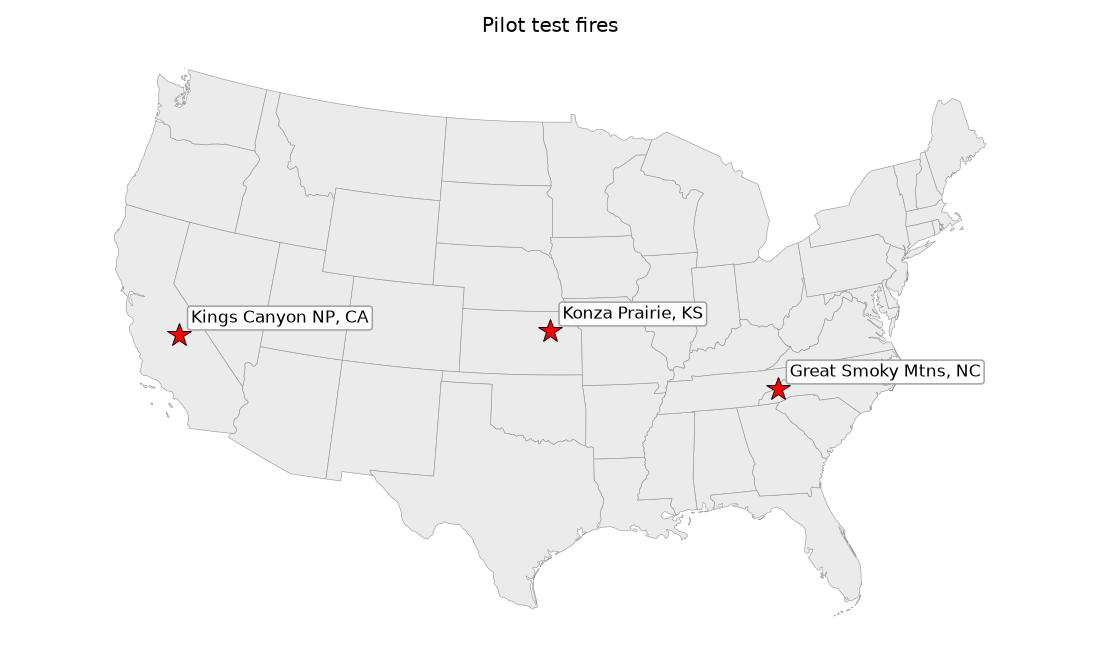
\includegraphics[keepaspectratio]{outputs/site_map.png}}
\caption{Map of the three pilot fires}
\end{figure}

\begin{longtable}[]{@{}
  >{\raggedright\arraybackslash}p{(\linewidth - 8\tabcolsep) * \real{0.2000}}
  >{\raggedright\arraybackslash}p{(\linewidth - 8\tabcolsep) * \real{0.2000}}
  >{\raggedright\arraybackslash}p{(\linewidth - 8\tabcolsep) * \real{0.2000}}
  >{\raggedright\arraybackslash}p{(\linewidth - 8\tabcolsep) * \real{0.2000}}
  >{\raggedright\arraybackslash}p{(\linewidth - 8\tabcolsep) * \real{0.2000}}@{}}
\toprule\noalign{}
\begin{minipage}[b]{\linewidth}\raggedright
Fire
\end{minipage} & \begin{minipage}[b]{\linewidth}\raggedright
Ecosystem
\end{minipage} & \begin{minipage}[b]{\linewidth}\raggedright
Recorded date
\end{minipage} & \begin{minipage}[b]{\linewidth}\raggedright
Size
\end{minipage} & \begin{minipage}[b]{\linewidth}\raggedright
Reference source and quality
\end{minipage} \\
\midrule\noalign{}
\endhead
\bottomrule\noalign{}
\endlastfoot
Konza Prairie, watershed K1B (KS) & Tallgrass prairie, burned every year
& Mar 22, 2019 & 445 ac & Konza LTER burned-watershed map. Strong: units
are bounded by roads and firebreaks, and burns usually fill them. \\
Cataloochee ``Short Bunk'' Rx, Great Smoky Mtns (NC) & Eastern oak/pine
forest, steep terrain & Apr 17, 2019 & 780 ac & National Park Service
perimeter, mapped with \textbf{differential GPS}. \\
Big Stump East Rx, Kings Canyon NP (CA) & Mixed conifer / giant sequoia,
closed canopy & Jun 23--28, 2025 & 119 ac & CAL FIRE prescribed-burn
layer (NPS record). Mapped acres match reported acres. \\
\end{longtable}

\subsection{Methods (plain English)}\label{methods-plain-english}

\subsubsection{What the method is given}\label{what-the-method-is-given}

To mimic a TNC-style record, each fire is reduced to: - a \textbf{point}
placed 290--400 m from the unit's center in a random direction (real
records are approximate), - the \textbf{recorded burn dates}, and - the
\textbf{reported acres}.

The reference perimeter is hidden from the mapping step and used only to
score it afterward.

\subsubsection{Free data used}\label{free-data-used}

\begin{longtable}[]{@{}
  >{\raggedright\arraybackslash}p{(\linewidth - 4\tabcolsep) * \real{0.3333}}
  >{\raggedright\arraybackslash}p{(\linewidth - 4\tabcolsep) * \real{0.3333}}
  >{\raggedright\arraybackslash}p{(\linewidth - 4\tabcolsep) * \real{0.3333}}@{}}
\toprule\noalign{}
\begin{minipage}[b]{\linewidth}\raggedright
Data
\end{minipage} & \begin{minipage}[b]{\linewidth}\raggedright
What it adds
\end{minipage} & \begin{minipage}[b]{\linewidth}\raggedright
Access
\end{minipage} \\
\midrule\noalign{}
\endhead
\bottomrule\noalign{}
\endlastfoot
\textbf{Sentinel-2} (10--20 m, \textasciitilde5-day revisit) & The main
burn signal. The ``Normalized Burn Ratio'' (NBR) compares near-infrared
and shortwave-infrared light; burning lowers it. \textbf{dNBR} is NBR
before minus NBR after. & Microsoft Planetary Computer, no key \\
\textbf{Sentinel-1 radar} & Sees through cloud and smoke & Planetary
Computer, no key \\
\textbf{VIIRS active fire} (375 m) & Independent confirmation that
something was burning & NASA FIRMS yearly archive, no key \\
\textbf{TESSERA embeddings} (10 m, annual) & AI summaries of each
pixel's whole year, from Sentinel-1 + Sentinel-2 & Source Cooperative,
no key \\
\end{longtable}

\subsubsection{Steps for each fire}\label{steps-for-each-fire}

\begin{enumerate}
\def\labelenumi{\arabic{enumi}.}
\tightlist
\item
  \textbf{Search window.} A square around the point, scaled to reported
  size (at least 5 km across).
\item
  \textbf{Clean Sentinel-2 images.} Every image from 60 days before to
  45 days after the burn is loaded. Clouds and cirrus are removed.
  Sentinel-2's own cloud-shadow label often mislabels fresh char as
  shadow, so that label is only trusted when a real cloud is nearby.
\item
  \textbf{Before and after.} For each pixel, NBR is taken from the 3
  clear looks just before the burn and the 3 just after. Their
  difference is dNBR.
\item
  \textbf{``When did it darken?''} This is the key addition. For each
  pixel, the method walks through \emph{every} clear image and finds the
  biggest drop in NBR that \textbf{persists} into the next clear image,
  so one-off glitches are ignored. That gives a date bracket for each
  pixel's change. A pixel is \textbf{date-matched} if that bracket
  overlaps the recorded burn dates (±2 days).
\item
  \textbf{Radar, VIIRS, and embeddings} are pulled for the same window.
\item
  \textbf{Draw the polygon.} Four methods are compared to show the
  omission/commission tradeoff. The figures and tables use these names:
\end{enumerate}

\begin{longtable}[]{@{}
  >{\raggedright\arraybackslash}p{(\linewidth - 2\tabcolsep) * \real{0.5000}}
  >{\raggedright\arraybackslash}p{(\linewidth - 2\tabcolsep) * \real{0.5000}}@{}}
\toprule\noalign{}
\begin{minipage}[b]{\linewidth}\raggedright
Name
\end{minipage} & \begin{minipage}[b]{\linewidth}\raggedright
What it maps
\end{minipage} \\
\midrule\noalign{}
\endhead
\bottomrule\noalign{}
\endlastfoot
\textbf{Standard} & Any pixel in the window with dNBR \textgreater{} 0.1
(a classic low-severity threshold). Ignores the point and date, the way
wall-to-wall burned-area products work. \\
\textbf{Near the point} & Pixels that darkened unusually \emph{compared
with the rest of the window} (handles regional green-up or drying), and
that are connected to the area within 1 km of the point. \\
\textbf{Near the point + date match} \emph{(main method)} & Same, but
each pixel must also have darkened on the recorded burn dates. \\
\textbf{+ embedding boost} & Same, plus weaker-signal pixels that are
date-matched \emph{and} show unusual embedding change. \\
\end{longtable}

All thresholds were set \textbf{before} looking at the results and are
the same for every fire. Nothing was tuned to these three. 7.
\textbf{Confidence and flags.} Each result gets a simple high/medium/low
rating plus plain flags, for example ``mapped area \textless{} 1/3 of
reported'' or ``no VIIRS detection''. A burn that isn't found is
reported as \textbf{not detected} rather than silently dropped.

\subsubsection{How results were scored}\label{how-results-were-scored}

Because the reference polygons are unit boundaries and low-intensity
burns are patchy, the scores focus on what can be trusted: -
\textbf{Detected?} At least 1 ha mapped inside the unit. - \textbf{False
detections outside the unit (ha).} Mapped area outside the unit and
outside every other recorded burn that year, with a 1-pixel edge
allowance. Prescribed fires rarely escape, so this is the most
trustworthy error number. - \textbf{Area mapped on other recorded burns
(ha).} Real fire, but the wrong event. - \textbf{\% of unit mapped as
burned.} An estimate of how much of the unit showed a signal. \emph{Not}
a miss rate. - \textbf{Signal strength.} For each data source: how well
does it tell the unit apart from clean background? (AUC: 0.5 = no better
than chance, 1.0 = perfect. Values well below 0.5 mean a strong signal
in the opposite direction.)

\subsection{Results}\label{results}

\begin{figure}
\centering
\pandocbounded{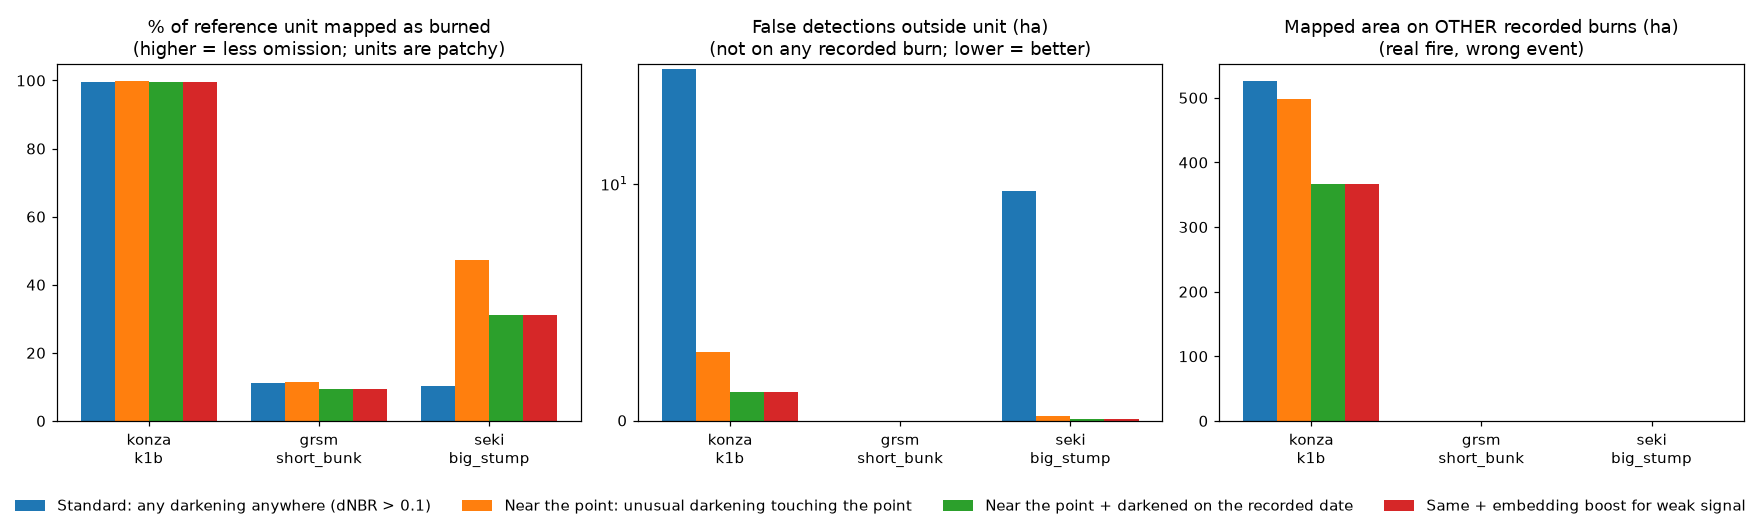
\includegraphics[keepaspectratio]{outputs/summary_tradeoff.png}}
\caption{Summary of the four methods}
\end{figure}

\subsubsection{Headline numbers (main method: near the point + date
match)}\label{headline-numbers-main-method-near-the-point-date-match}

\begin{longtable}[]{@{}
  >{\raggedright\arraybackslash}p{(\linewidth - 10\tabcolsep) * \real{0.1667}}
  >{\raggedright\arraybackslash}p{(\linewidth - 10\tabcolsep) * \real{0.1667}}
  >{\raggedright\arraybackslash}p{(\linewidth - 10\tabcolsep) * \real{0.1667}}
  >{\raggedright\arraybackslash}p{(\linewidth - 10\tabcolsep) * \real{0.1667}}
  >{\raggedright\arraybackslash}p{(\linewidth - 10\tabcolsep) * \real{0.1667}}
  >{\raggedright\arraybackslash}p{(\linewidth - 10\tabcolsep) * \real{0.1667}}@{}}
\toprule\noalign{}
\begin{minipage}[b]{\linewidth}\raggedright
Fire
\end{minipage} & \begin{minipage}[b]{\linewidth}\raggedright
Detected?
\end{minipage} & \begin{minipage}[b]{\linewidth}\raggedright
\% of unit mapped
\end{minipage} & \begin{minipage}[b]{\linewidth}\raggedright
False detections outside unit
\end{minipage} & \begin{minipage}[b]{\linewidth}\raggedright
Same number for \textbf{Standard} method
\end{minipage} & \begin{minipage}[b]{\linewidth}\raggedright
VIIRS confirms?
\end{minipage} \\
\midrule\noalign{}
\endhead
\bottomrule\noalign{}
\endlastfoot
Konza prairie & Yes & 99.7\% & 1.2 ha & 34.6 ha & Yes (4 detections,
nearest 284 m from point) \\
Smokies oak/pine & Yes & 9.4\% & 0 ha & 0 ha & No \\
Kings Canyon conifer & Yes & 31\% & 0.1 ha & 9.7 ha & Yes (1 detection,
447 m from point) \\
\end{longtable}

\textbf{1. All three burns were found}, including both under-canopy
burns, from an approximate point and a date. No false detections showed
up outside the units with the main method.

\textbf{2. Using the point and the date cuts false detections sharply.}
Compared with the standard method, false detections fell from 34.6 to
1.2 ha at Konza and from 9.7 to 0.1 ha in Kings Canyon. This is the
omission/commission problem raised in the discussion: starting from
recorded points and dates avoids most of it.

\textbf{3. The grassland is easy. Under-canopy forest burns are partly
visible.} - \emph{Konza:} essentially the whole unit shows a strong burn
signal (dNBR separates it from background almost perfectly, AUC 0.996).
- \emph{Kings Canyon:} about a third to a half of the unit shows a
signal (31\% with the date match; 47\% with the near-the-point method).
- \emph{Smokies:} only about 10\% of the unit. The reference unit
includes unburned patches, so the true burned fraction is unknown. That
is why field estimates of percent burned would be valuable.

\textbf{4. Spring green-up hides eastern understory burns, and the
``when did it darken?'' step helps.} In the Smokies, leaf-out between
the before and after images raised NBR across the landscape. That masked
the burn: simple dNBR did \emph{no better than chance} at separating the
unit from background (AUC 0.43). The per-pixel timing approach did
better (AUC 0.74). The approach was built for exactly this case, but the
signal is still weak.

\textbf{5. Date matching can separate burns about 10 days apart, but not
2--4 days apart.} Konza recorded 36 other burned areas in 2019, on dates
from February to November, which gave a natural test: - Watersheds
burned \textbf{10 or more days} from the target: ≤1\% of their pixels
were wrongly matched to the target date. - Neighbors burned \textbf{2--4
days earlier}: 27--93\% were matched to the target date, because
Sentinel-2 had no clear image in between. That is why the main method
maps 367 ha of neighboring burns at Konza (real fire, wrong event).
Daily imagery such as Planet would separate these, which is a concrete,
well-defined use for the remaining Planet credits.

\textbf{6. Radar helps in grassland, not under trees.} Sentinel-1 showed
a clear backscatter drop in the burned prairie (about −0.8 dB; AUC 0.11
for VV, i.e., strong separation in the negative direction). It showed
nothing useful in either forest (AUC 0.42--0.53). This is C-band radar;
L-band radar (NISAR), which reaches through canopy, was not tested.

\textbf{7. VIIRS confirmed 2 of 3 burns,} and not the Smokies burn. As
expected, a missing VIIRS detection is not evidence that no burn
happened.

\textbf{8. Embeddings: the obvious use failed, a different use looked
promising.} - \emph{Year-over-year embedding change} did \textbf{not}
work. At Konza the unit changed \emph{less} than the background (AUC
0.14), because K1B burns every year, so 2018 and 2019 look alike. In the
forests it was at chance (0.44--0.52). The embedding boost added at most
0.4 ha anywhere. - \emph{A classifier on the burn-year embeddings},
trained only on the \emph{other} recorded Konza burns, picked out the
held-out K1B unit well (AUC 0.93; 90\% of unit pixels flagged). It also
flagged 21\% of nearby unburned prairie, and annual embeddings carry no
burn date. In the two forests there were no other recorded burns nearby
to train on, so this couldn't be tested. Embeddings look like a useful
\textbf{supporting layer}, not a primary mapper.

\textbf{9. Confidence flags behaved sensibly.} All three were rated
``medium''. Konza was flagged ``mapped area \textgreater{} 2×
reported'', which correctly pointed to the neighboring burns. Both
forest burns were flagged ``mapped area \textless{} 1/3 of reported'',
and the Smokies burn was also flagged ``no VIIRS detection''.

\subsubsection{Per-fire figures}\label{per-fire-figures}

Each figure shows: before and after images, the burn signal, when each
pixel darkened, radar change, embedding change, the standard method, and
the main method. The cyan outline is the reference unit, the yellow star
is the simulated input point, and dashed white outlines are other
recorded burns. Each panel has a scale bar. The small US map in the
top-left corner marks the fire (red star), and its coordinates are in
the title.

\pandocbounded{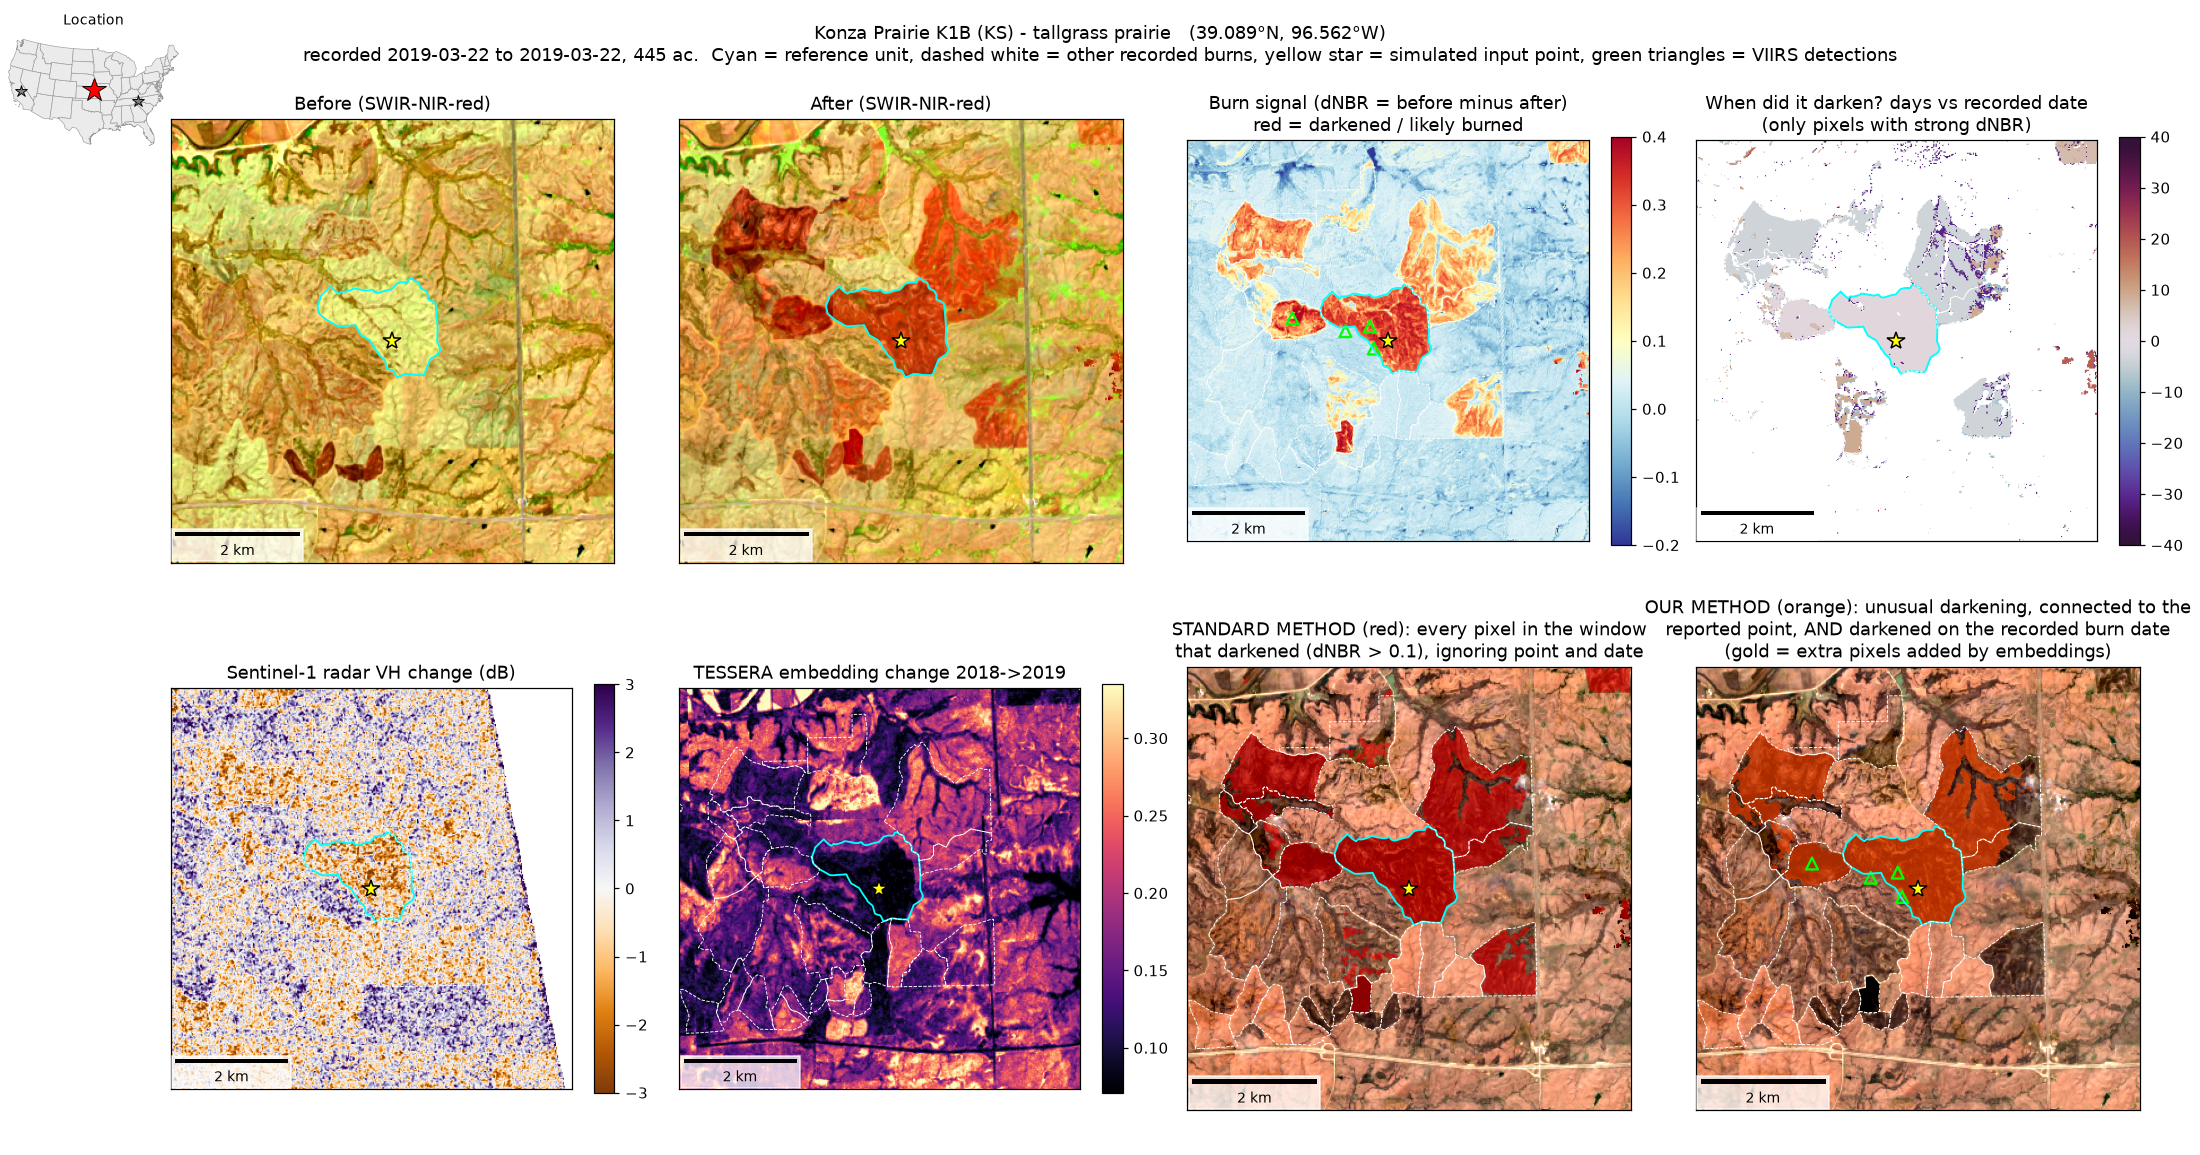
\includegraphics[keepaspectratio]{outputs/konza_k1b/konza_k1b_panels.png}}
\pandocbounded{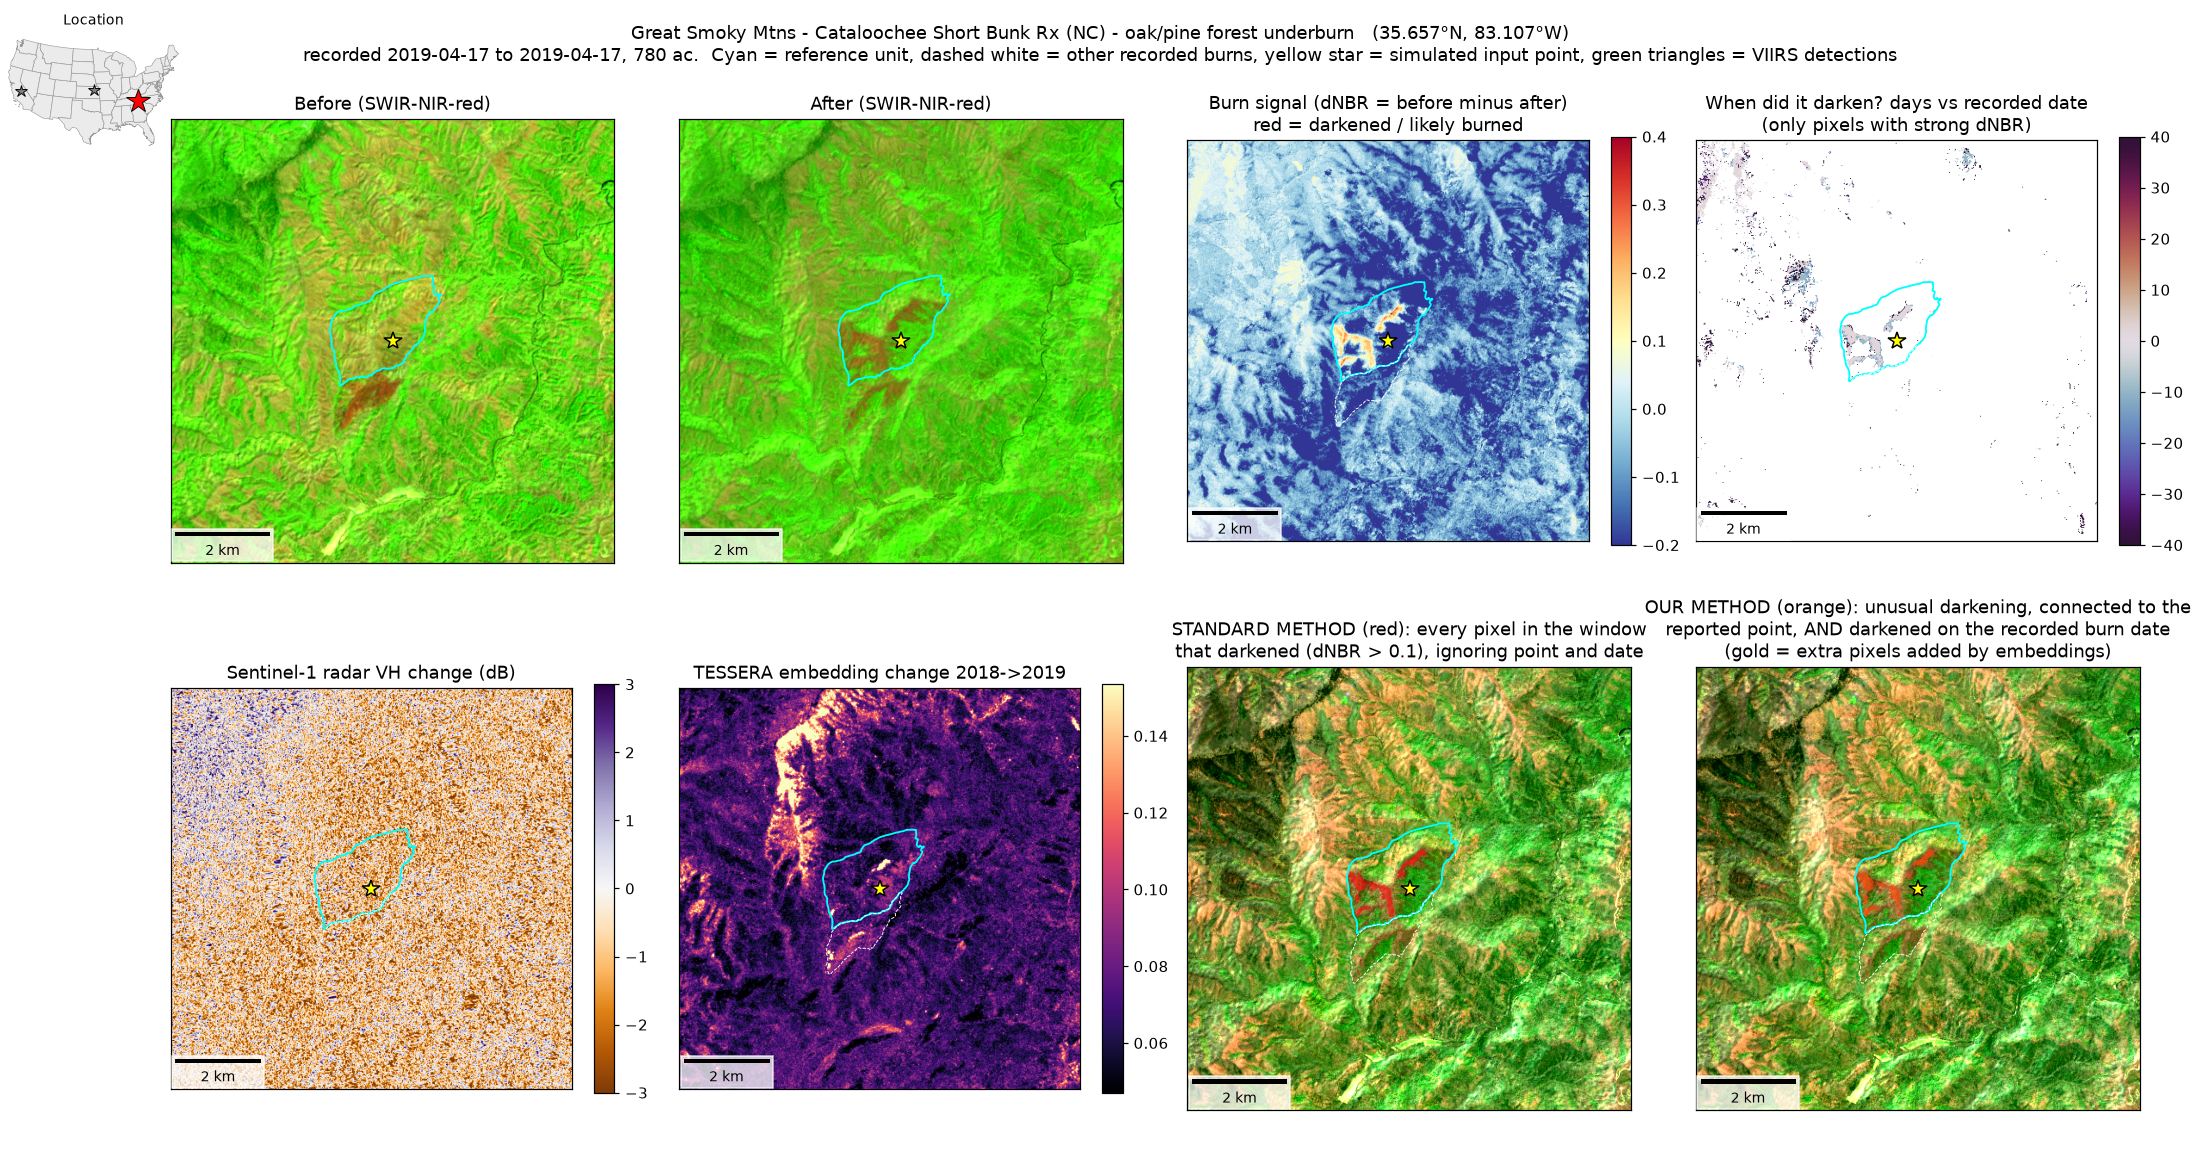
\includegraphics[keepaspectratio]{outputs/grsm_short_bunk/grsm_short_bunk_panels.png}}
\pandocbounded{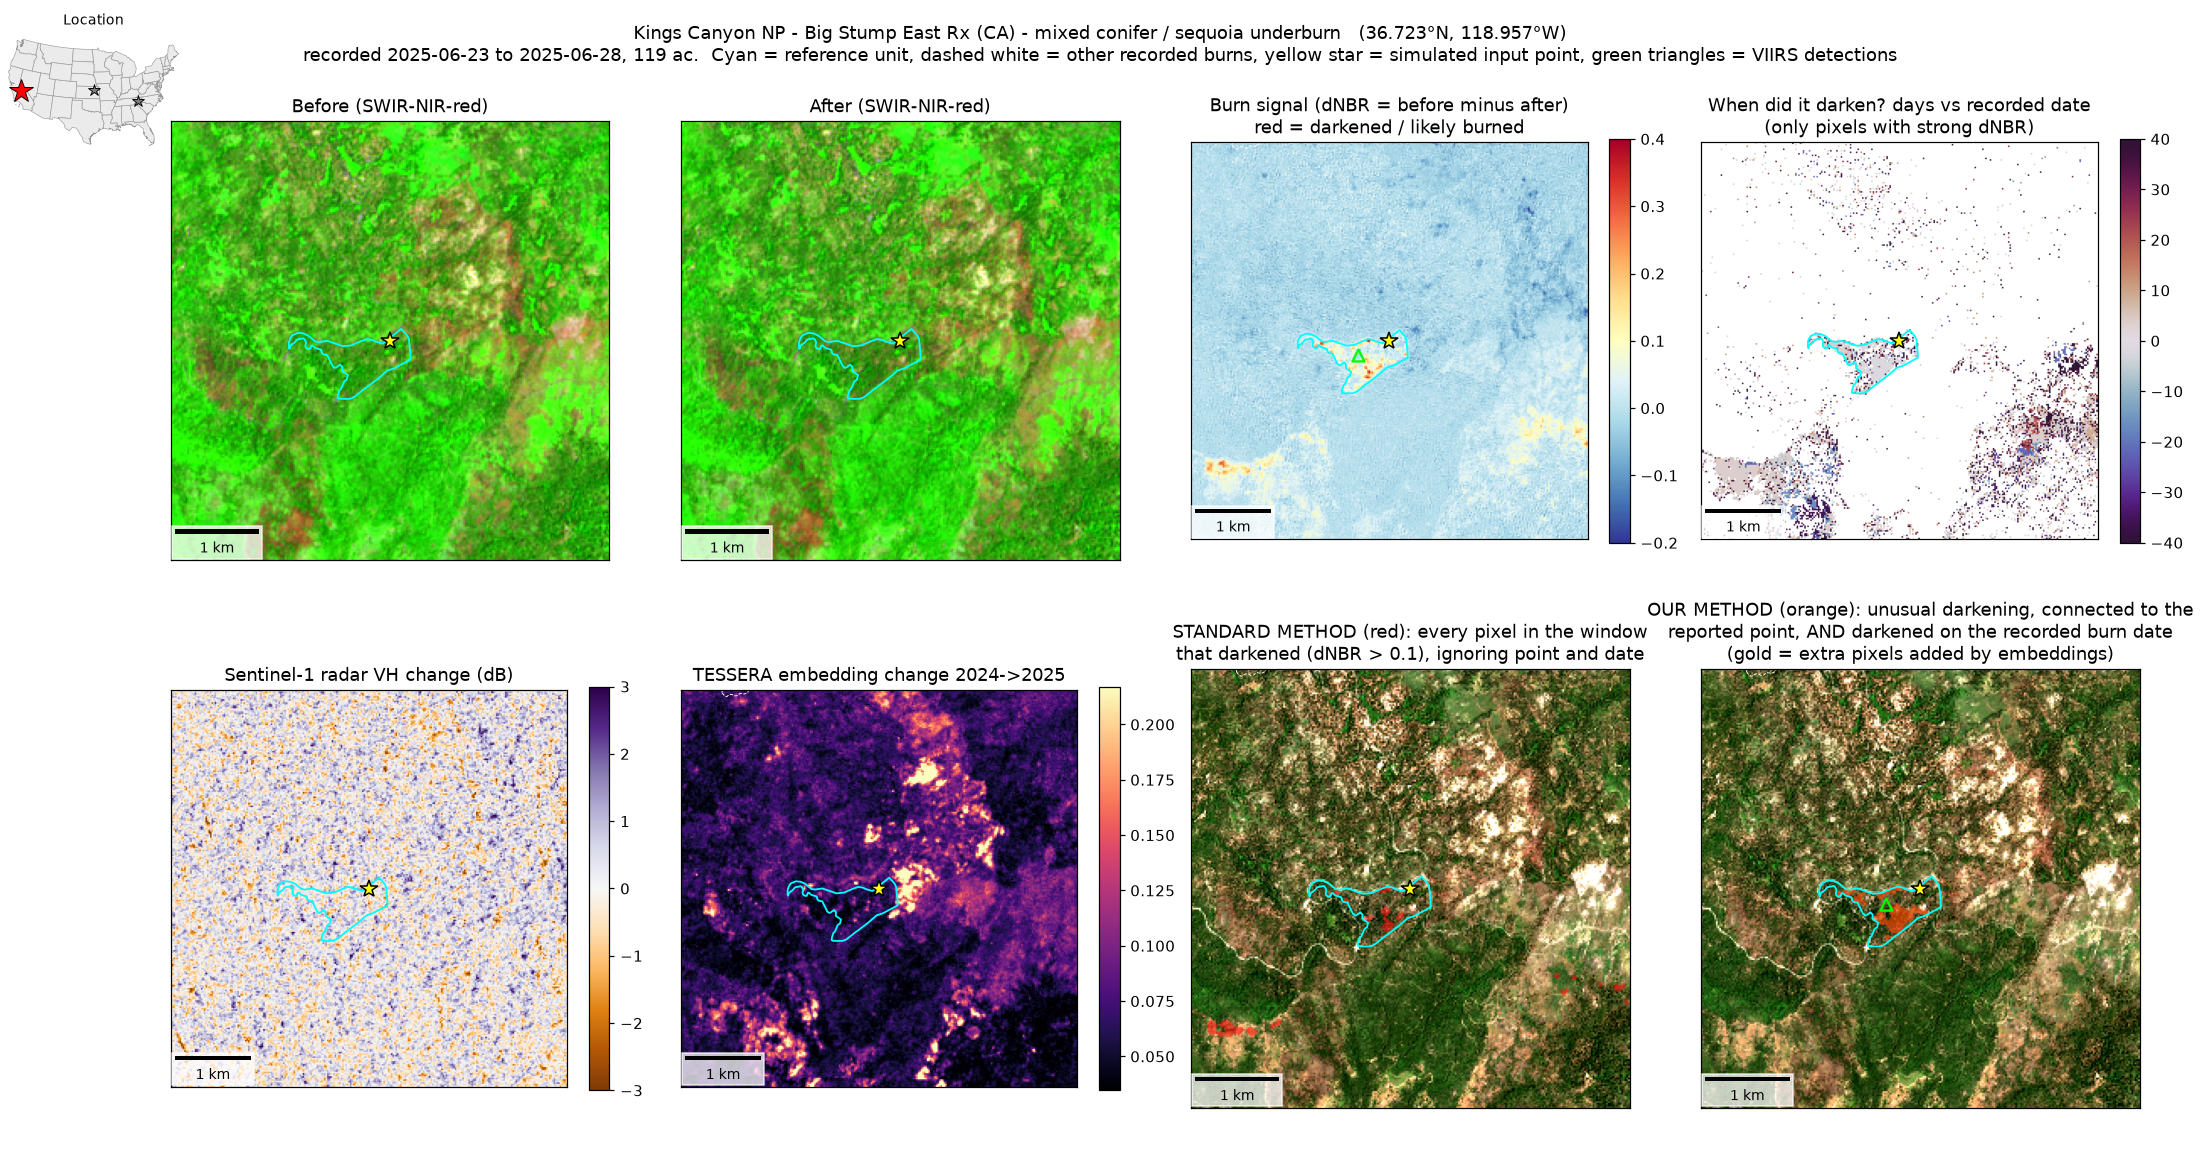
\includegraphics[keepaspectratio]{outputs/seki_big_stump/seki_big_stump_panels.png}}

\subsection{Round 2: 22 fires, fully automatic, with and without
snapping}\label{round-2-22-fires-fully-automatic-with-and-without-snapping}

\subsubsection{Why round 2}\label{why-round-2}

Round 1 left three open questions. First, does the method hold up beyond
three hand-picked fires? Second, can the spring green-up problem in
eastern forests be fixed? Third, do control lines (the roads, trails,
and streams that bound most burn units) help draw better edges? Round 2
tests all three. It follows the rule that \textbf{nothing is done by
hand}, so it could be run on hundreds of points.

\subsubsection{How the 22 fires were chosen
(automatically)}\label{how-the-22-fires-were-chosen-automatically}

The fires were picked by a fixed rule, not by looking at imagery:

\begin{itemize}
\tightlist
\item
  The three round-1 fires, plus
\item
  National Park Service prescribed burns from the public NPS fire
  perimeter service that were \textbf{mapped with GPS}, 60--1,200 acres,
  lasting 4 days or less, and not pile burns. At most one burn per park
  and five per NPS region were taken, largest first.
\end{itemize}

That rule produced 19 NPS burns. All are from 2019, because the public
NPS layer only contains prescribed-fire records for that year. All the
imagery and terrain data exist for 2019. The one exception is the road,
trail, and stream layer, which is current (2026) rather than 2019. Most
control lines are permanent, so this matters little, but a new road
could create a false edge.

Each fire again gets a simulated input point placed a few hundred meters
from the unit center.

\begin{figure}
\centering
\pandocbounded{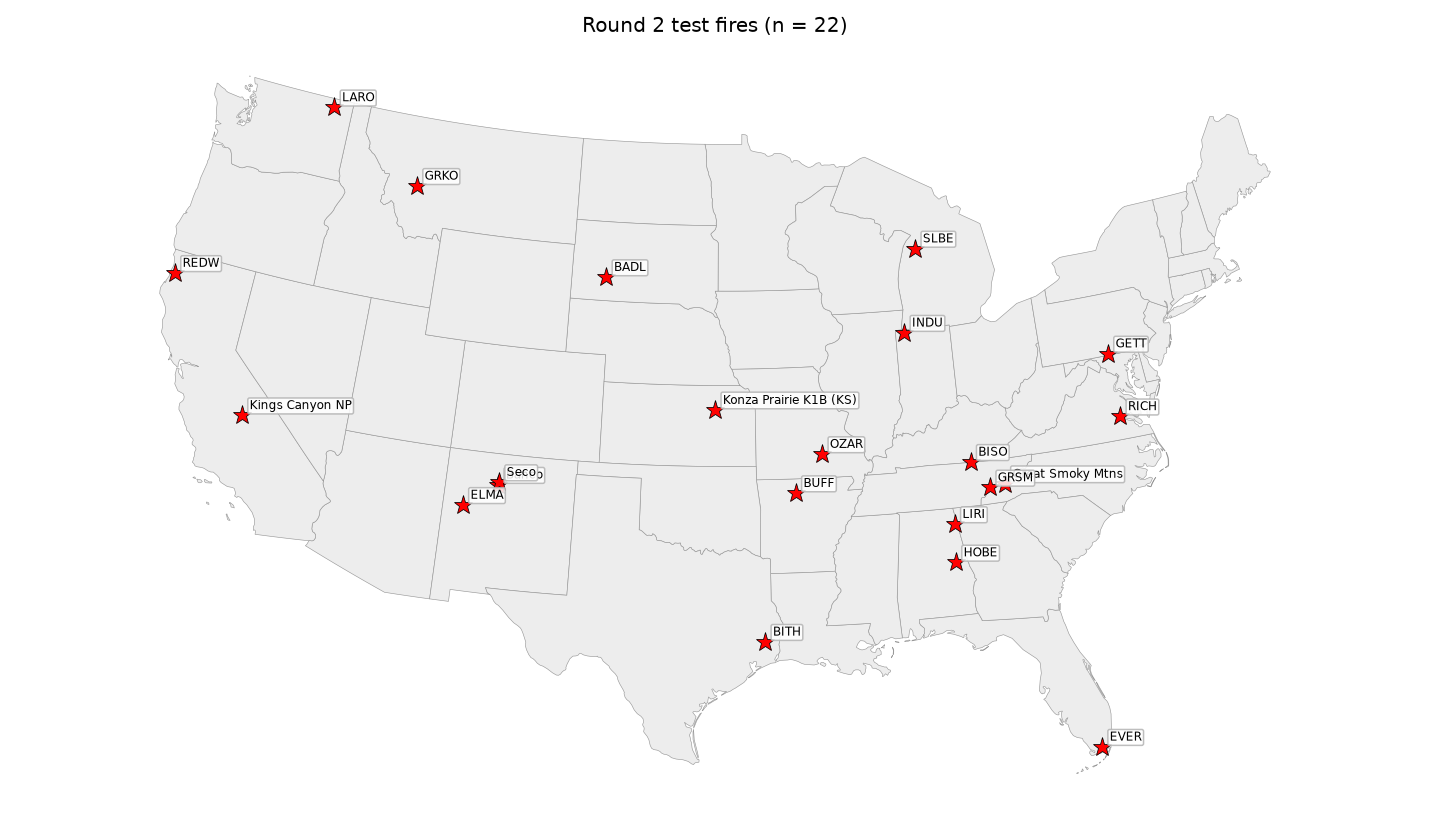
\includegraphics[keepaspectratio]{outputs_v2/site_map_round2.png}}
\caption{Map of the 22 round-2 fires}
\end{figure}

Land cover, from ESA WorldCover tree share inside each unit, splits the
sample into \textbf{14 forest} (\textgreater70\% trees), \textbf{2
mixed}, and \textbf{6 open} (\textless30\% trees) fires. One open unit
is an Everglades wetland (77\% wetland).

\subsubsection{What was added in round
2}\label{what-was-added-in-round-2}

\begin{enumerate}
\def\labelenumi{\arabic{enumi}.}
\tightlist
\item
  \textbf{Landsat 8 added to Sentinel-2.} More clear looks means a
  tighter date bracket for each pixel. Landsat shortened the gap between
  the burn and the first clear look after it at several cloudy sites,
  for example Big South Fork (13 to 4 days) and Horseshoe Bend (14 to 10
  days). Some sites were still cloudy for weeks: the first clear look
  came 38 days after the burn at Little River Canyon, 19 at Ozark
  Riverways, and 16 at Buffalo River.
\item
  \textbf{Green-up correction using look-alike pixels.} In round 1, each
  pixel was compared with the whole window, which fails when forests
  leaf out unevenly across terrain. In round 2, every pixel is compared
  only with pixels of the \textbf{same kind} that are well away from the
  burn. ``Same kind'' comes from the previous year's TESSERA embeddings,
  grouped into 30 types (for example, north-facing oak forest or open
  pasture). On each image date, the typical NBR change of that type's
  distant pixels is subtracted. What remains is change that the
  surrounding landscape did \emph{not} also go through. This is a new
  use for the embeddings: they don't detect fire, but they define fair
  comparisons.
\item
  \textbf{Control lines, from free national data.} Roads, trails,
  streams, water edges, and power lines come from \textbf{Overture Maps}
  (a free, open, cloud-hosted version of OpenStreetMap and other
  sources). Ridgelines come from the \textbf{Copernicus 30 m elevation
  model}. Together these lines cut the landscape into \textbf{cells},
  much as burn units are laid out.
\item
  \textbf{Snapping (optional step).} For each cell no more than 3× the
  reported burn size:

  \begin{itemize}
  \tightlist
  \item
    if at least 40\% of the cell was mapped as burned, the \textbf{whole
    cell is filled};
  \item
    if less than 10\% was mapped, those few pixels are \textbf{removed}
    as likely noise;
  \item
    otherwise the mapped pixels are kept as they are.
  \end{itemize}

  All of these numbers were set before seeing any results and are the
  same for every fire.
\end{enumerate}

\subsubsection{The five versions
compared}\label{the-five-versions-compared}

\begin{longtable}[]{@{}
  >{\raggedright\arraybackslash}p{(\linewidth - 2\tabcolsep) * \real{0.5000}}
  >{\raggedright\arraybackslash}p{(\linewidth - 2\tabcolsep) * \real{0.5000}}@{}}
\toprule\noalign{}
\begin{minipage}[b]{\linewidth}\raggedright
Name in figures
\end{minipage} & \begin{minipage}[b]{\linewidth}\raggedright
What it is
\end{minipage} \\
\midrule\noalign{}
\endhead
\bottomrule\noalign{}
\endlastfoot
\textbf{Standard} & Any darkening (dNBR \textgreater{} 0.1) anywhere in
the window. Ignores the point and date. \\
\textbf{Round 1} & The round-1 main method: Sentinel-2 only, near the
point, darkened on the recorded date. \\
\textbf{Round 1 + snap} & Round 1, then snapped to control lines. \\
\textbf{Round 2} & Sentinel-2 + Landsat, green-up correction with
look-alike pixels, near the point, darkened on the recorded date. \\
\textbf{Round 2 + snap} & Round 2, then snapped to control lines. \\
\end{longtable}

Scoring is the same as in round 1. One measure was added: a
\textbf{solid detection}, meaning at least 10\% of the unit was mapped.
A detection of only 1 ha in a 300 ha unit is real but not useful as a
polygon.

\subsubsection{Round 2 results}\label{round-2-results}

\begin{figure}
\centering
\pandocbounded{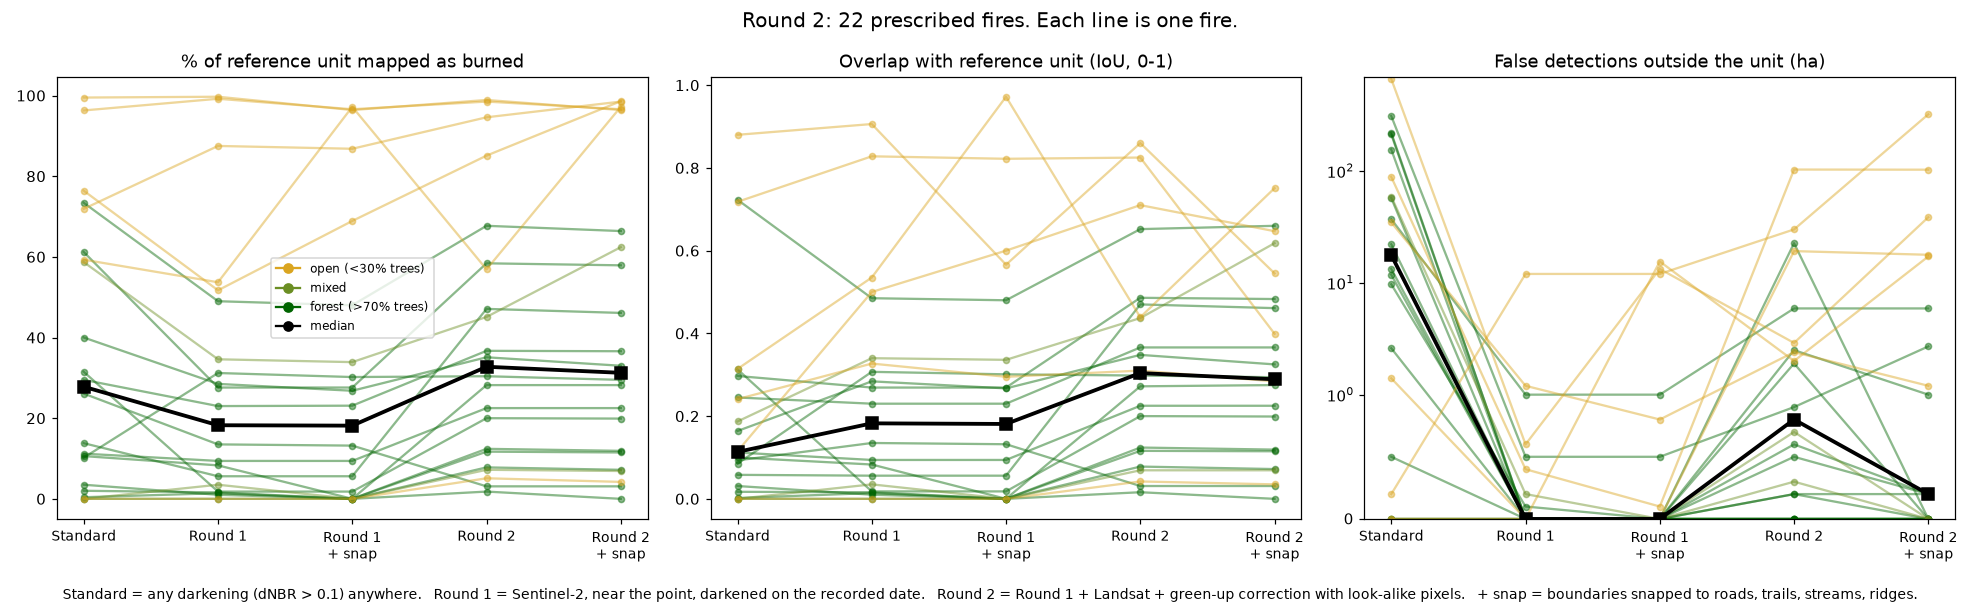
\includegraphics[keepaspectratio]{outputs_v2/summary_round2.png}}
\caption{Round 2 summary}
\end{figure}

\begin{longtable}[]{@{}
  >{\raggedright\arraybackslash}p{(\linewidth - 12\tabcolsep) * \real{0.1429}}
  >{\raggedright\arraybackslash}p{(\linewidth - 12\tabcolsep) * \real{0.1429}}
  >{\raggedright\arraybackslash}p{(\linewidth - 12\tabcolsep) * \real{0.1429}}
  >{\raggedright\arraybackslash}p{(\linewidth - 12\tabcolsep) * \real{0.1429}}
  >{\raggedright\arraybackslash}p{(\linewidth - 12\tabcolsep) * \real{0.1429}}
  >{\raggedright\arraybackslash}p{(\linewidth - 12\tabcolsep) * \real{0.1429}}
  >{\raggedright\arraybackslash}p{(\linewidth - 12\tabcolsep) * \real{0.1429}}@{}}
\toprule\noalign{}
\begin{minipage}[b]{\linewidth}\raggedright
Version
\end{minipage} & \begin{minipage}[b]{\linewidth}\raggedright
Detected (≥1 ha in unit)
\end{minipage} & \begin{minipage}[b]{\linewidth}\raggedright
Solid detection (≥10\% of unit)
\end{minipage} & \begin{minipage}[b]{\linewidth}\raggedright
Median \% of unit mapped
\end{minipage} & \begin{minipage}[b]{\linewidth}\raggedright
Median overlap (IoU)
\end{minipage} & \begin{minipage}[b]{\linewidth}\raggedright
Total false detections outside units
\end{minipage} & \begin{minipage}[b]{\linewidth}\raggedright
Fires with \textgreater5 ha false
\end{minipage} \\
\midrule\noalign{}
\endhead
\bottomrule\noalign{}
\endlastfoot
Standard & 18 of 22 & 16 & 28\% & 0.11 & 1,897 ha & 14 \\
Round 1 & 20 & 12 & 18\% & 0.18 & 16 ha & 1 \\
Round 1 + snap & 15 & 12 & 18\% & 0.18 & 43 ha & 3 \\
\textbf{Round 2} & \textbf{22} & \textbf{17} & \textbf{33\%} &
\textbf{0.30} & 196 ha & 5 \\
Round 2 + snap & 21 & 17 & 31\% & 0.29 & 509 ha & 6 \\
\end{longtable}

Median \% of unit mapped, by land cover:

\begin{longtable}[]{@{}
  >{\raggedright\arraybackslash}p{(\linewidth - 10\tabcolsep) * \real{0.1667}}
  >{\raggedright\arraybackslash}p{(\linewidth - 10\tabcolsep) * \real{0.1667}}
  >{\raggedright\arraybackslash}p{(\linewidth - 10\tabcolsep) * \real{0.1667}}
  >{\raggedright\arraybackslash}p{(\linewidth - 10\tabcolsep) * \real{0.1667}}
  >{\raggedright\arraybackslash}p{(\linewidth - 10\tabcolsep) * \real{0.1667}}
  >{\raggedright\arraybackslash}p{(\linewidth - 10\tabcolsep) * \real{0.1667}}@{}}
\toprule\noalign{}
\begin{minipage}[b]{\linewidth}\raggedright
Cover
\end{minipage} & \begin{minipage}[b]{\linewidth}\raggedright
Standard
\end{minipage} & \begin{minipage}[b]{\linewidth}\raggedright
Round 1
\end{minipage} & \begin{minipage}[b]{\linewidth}\raggedright
Round 1 + snap
\end{minipage} & \begin{minipage}[b]{\linewidth}\raggedright
Round 2
\end{minipage} & \begin{minipage}[b]{\linewidth}\raggedright
Round 2 + snap
\end{minipage} \\
\midrule\noalign{}
\endhead
\bottomrule\noalign{}
\endlastfoot
Forest (14 fires) & 12.5\% & 8.9\% & 7.5\% & 25.4\% & 25.4\% \\
Mixed (2) & 29\% & 19\% & 17\% & 26\% & 35\% \\
Open (6) & 74\% & 71\% & 92\% & 90\% & 97\% \\
\end{longtable}

Solid detections in forest: 10 of 14 for Standard, 6 for Round 1, and
\textbf{11 for Round 2}.

\textbf{1. Round 2 found every burn and roughly tripled the useful
signal in forests.} All 22 burns were detected. In forest units, the
median share mapped rose from 9\% (round 1) to 25\%. The largest gains
came at eastern and southern forest sites where green-up or cloud had
hidden the burn:

\begin{longtable}[]{@{}lll@{}}
\toprule\noalign{}
Fire & Round 1 & Round 2 \\
\midrule\noalign{}
\endhead
\bottomrule\noalign{}
\endlastfoot
Ozark Riverways, Devils Well (MO) & 5.6\% & 47\% \\
Horseshoe Bend, NW Complex (AL) & 1.6\% & 28\% \\
Bandelier, Banco North (NM) & 1.8\% & 20\% \\
Buffalo River, Cash Bend (AR) & 1.0\% & 12\% \\
Smokies, Short Bunk (NC) (round-1 fire) & 9.4\% & 22.5\% \\
Smokies, Maple Branch (TN) & 52\% & 85\% \\
\end{longtable}

\textbf{2. It costs some false detections, but far fewer than the
standard method.} False detections outside units rose from 16 ha (round
1) to 196 ha (round 2). The standard method had 1,897 ha. Most of the
round 2 increase came from four fires: Everglades (103 ha), Badlands (30
ha), El Malpais (23 ha), and Grant-Kohrs Ranch (19 ha). In the
Everglades, the ``false'' area is next to a large burn in a landscape
that burns often, so much of it is probably real fire that wasn't in the
NPS layer. That can't be confirmed without other records. The median
fire had essentially no false detections (under 0.5 ha in forest and
mixed units).

\textbf{3. One fire got worse.} At Big Thicket, Sandhill (TX) the share
mapped fell from 13.5\% to 3\%. The look-alike correction removed signal
there. One possible reason is that the comparison pixels of the same
type were also darkening (for example, from unrecorded burns or drying
in the same pine type), but this wasn't diagnosed. A larger sample would
show how often this happens.

\textbf{4. Snapping to control lines helps in some places and hurts in
others.} - \textbf{Where it helps:} units bounded by roads, canals, and
streams, where the burn fills the unit. In the Everglades wetland unit,
snapping raised the overlap with the reference from 0.54 to 0.97 (97\%
of the unit mapped). It also helped at Smokies Maple Branch (85\% to
99\%), Lake Roosevelt (overlap 0.44 to 0.62), and the open-cover class
overall (median 90\% to 97\%). - \textbf{Where it hurts:} - \emph{Big
open cells.} At Badlands, a large prairie cell bordered by few lines was
filled, adding about 290 ha of false area. - \emph{Cells that don't
match the unit.} At Richmond (Malvern Hill), snapping lowered the
overlap from 0.91 to 0.57. - \emph{Weak, patchy burns.} The ``remove
cells under 10\%'' rule erased real but faint detections. In round 1,
snapping cut detections from 20 to 15 fires (Little River Canyon,
Sleeping Bear Dunes, Horseshoe Bend, and Buffalo River all dropped to
zero). With round 2's stronger signal, snapping lost only one (El
Malpais). - \textbf{Bottom line:} with this free line data, snapping
does not improve results on average (median overlap 0.30 without, 0.29
with) and it raises false detections. It is worth using as a
\textbf{second product}, or only where the mapped burn already fills
most of a closed cell, not as a default. Real burn-unit boundaries, if
TNC or partners have them, would likely work much better than generic
roads and streams.

\textbf{5. Wetlands can be mapped.} The Everglades burn (77\% wetland)
was found with both rounds and mapped almost perfectly after snapping.
This supports \emph{not} masking wetlands out. The colleague's point
that wetlands burn after dry spells holds, and the method can see them.

\textbf{6. Grasslands and open woodlands remain easy. Under-canopy
forest burns remain the hard part.} Five of six open units were solidly
detected by every method. The exception, Grant-Kohrs Ranch (MT), showed
only about 5\% even in round 2. In forest, round 2 brings most burns to
a usable level, but a quarter of the unit mapped is typical. Whether
that reflects the method or real patchiness of the burn can't be told
without field data.

\subsubsection{Example round-2 figures}\label{example-round-2-figures}

Each figure shows the after-burn image, the round-1 burn signal, the
round-2 (green-up-corrected) burn signal, and the mapped polygons for
round 1, round 2, and round 2 with snapping. Control lines are drawn in
light grey. Each panel has a scale bar, and the small US map marks the
fire.

\emph{Ozark Riverways: a forest burn hidden by green-up in round 1 and
recovered in round 2.}
\pandocbounded{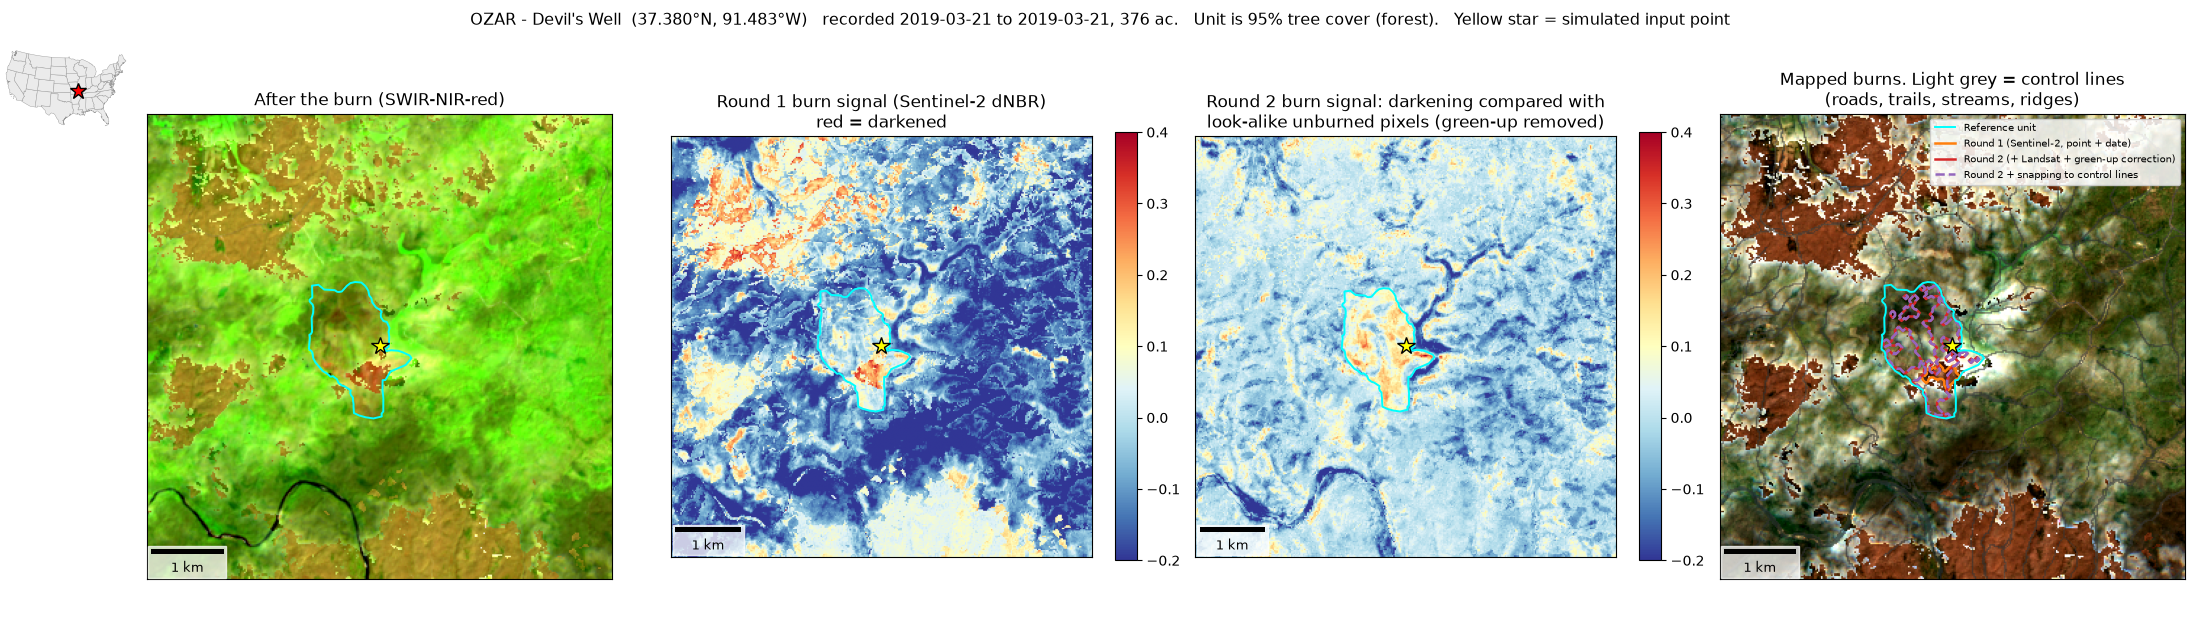
\includegraphics[keepaspectratio]{outputs_v2/nps_OZAR_devilswell/nps_OZAR_devilswell_panels.png}}

\emph{Everglades: a wetland burn where snapping to canals and roads
works very well.}
\pandocbounded{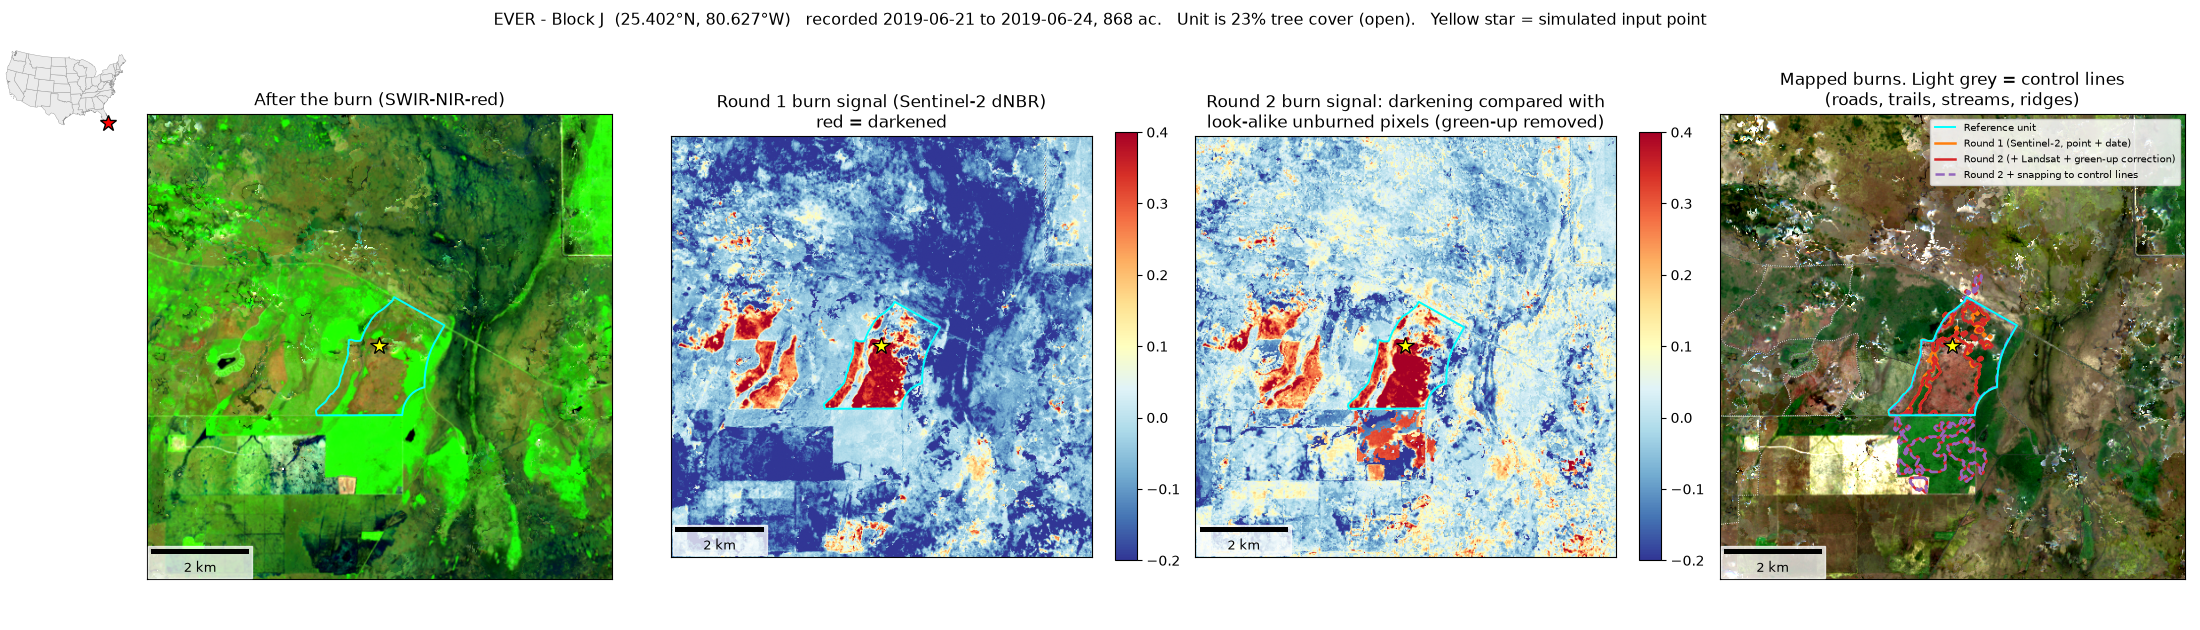
\includegraphics[keepaspectratio]{outputs_v2/nps_EVER_blockj/nps_EVER_blockj_panels.png}}

\emph{Badlands: a prairie burn where snapping fills a large open cell
and overshoots.}
\pandocbounded{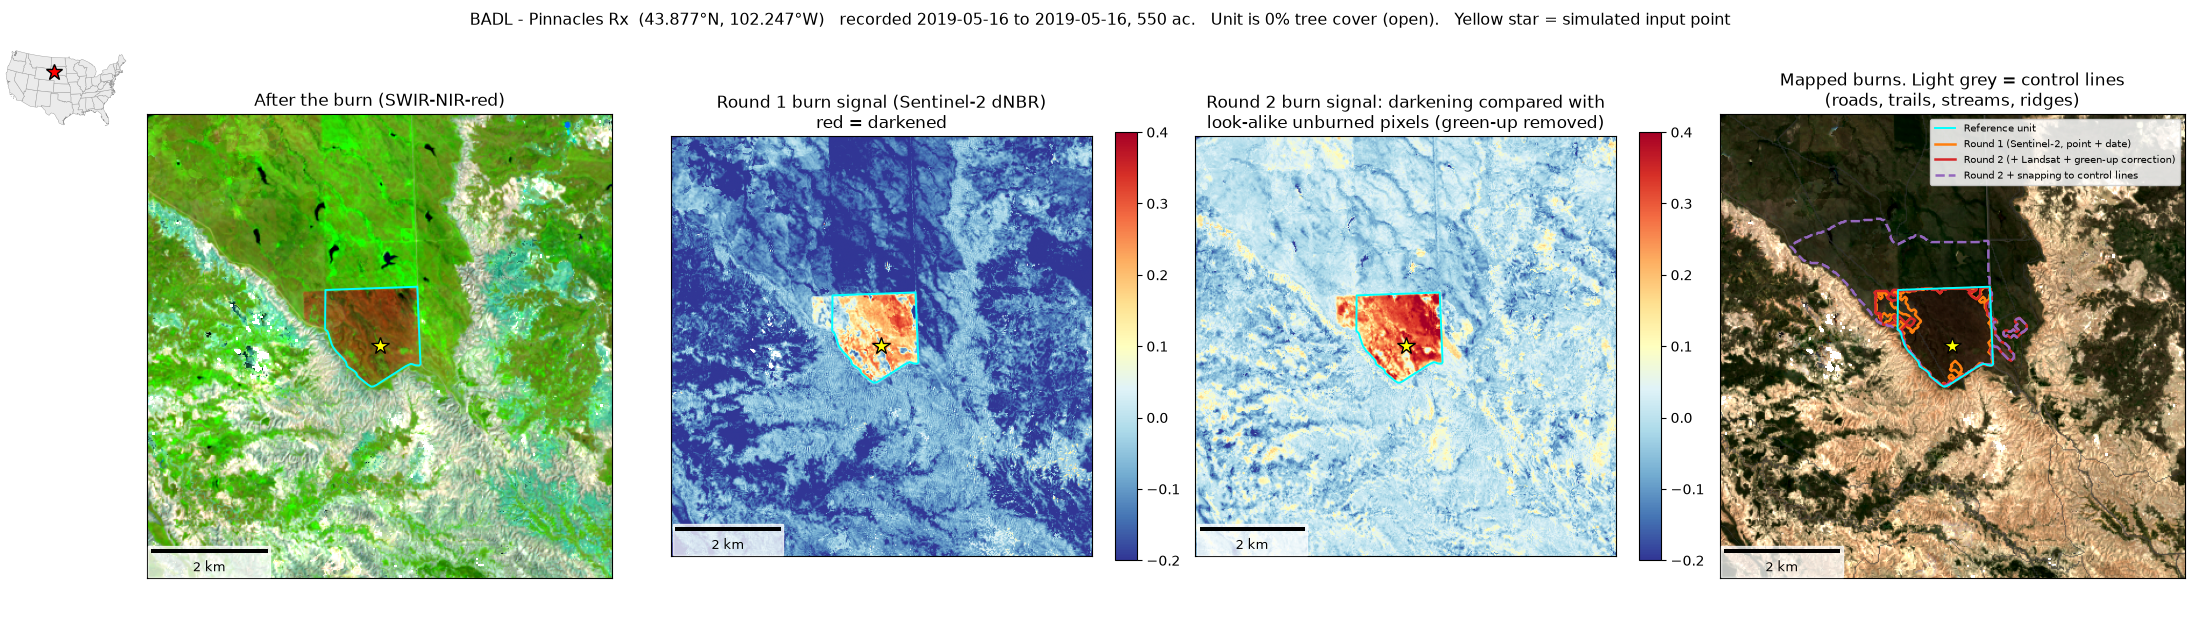
\includegraphics[keepaspectratio]{outputs_v2/nps_BADL_pinnaclesrx/nps_BADL_pinnaclesrx_panels.png}}

Figures for all 22 fires are in
\texttt{outputs\_v2/\textless{}fire\textgreater{}/\textless{}fire\textgreater{}\_panels.png}.
Per-fire numbers are in \texttt{outputs\_v2/metrics\_round2.csv}.

\subsubsection{A replicability lesson from round
2}\label{a-replicability-lesson-from-round-2}

The first version of the control-line step used the public OpenStreetMap
query service (Overpass). It was rate-limited and refused requests
partway through the batch, and a backup server was down. It was replaced
with \textbf{Overture Maps}, which is read directly from cloud storage
with no server to overload. That fixed it. For hundreds of points, every
data source should be a bulk, cloud-hosted file (Planetary Computer,
Source Cooperative, Overture), not a shared query service.

\subsection{Caveats}\label{caveats}

\begin{itemize}
\tightlist
\item
  \textbf{Small samples.} Three fires in round 1, 22 in round 2 (only 2
  in the mixed class). These show patterns, not program-wide accuracy.
\item
  \textbf{References are unit boundaries.} ``\% of unit mapped''
  understates performance by an unknown amount when burns are patchy.
\item
  \textbf{``False detections'' may be real fires.} Burns not in the
  reference layers count as false, which likely inflates the Everglades
  number in particular.
\item
  \textbf{Round 2 uses 2019 fires} because that's what the public NPS
  layer contains. Sentinel-2, Landsat 8, TESSERA, elevation, and land
  cover all cover 2019. Control lines are a 2026 snapshot.
\item
  \textbf{Settings were fixed in advance and not tuned.} Some of them
  (for example the 40\% and 10\% snapping cutoffs and the 3× cell-size
  limit) are guesses that a larger sample could improve.
\item
  \textbf{Wetlands:} only one wetland burn was tested (Everglades), and
  it worked. Northeastern wetlands burned after dry spells still need
  their own test fires.
\item
  \textbf{The confidence rating is a simple rule-of-thumb score}, not a
  calibrated probability.
\item
  \textbf{Data quirks handled in code:} Sentinel-2 images after January
  2022 need a reflectance offset removed. TESSERA only publishes an
  index for 2024, so the code builds index rows for other years from the
  file headers. The TESSERA reader needs \texttt{xarray==2025.6.1} with
  \texttt{zarr\textless{}3}.
\end{itemize}

\subsection{Is this replicable for hundreds of
points?}\label{is-this-replicable-for-hundreds-of-points}

Yes, and round 2 showed it in practice. All 22 fires ran unattended from
the input record alone (point, dates, acres), with no accounts, keys, or
hand edits. Every data source is free and cloud-hosted: Planetary
Computer (Sentinel-2, Landsat, elevation, land cover), Source
Cooperative (TESSERA), Overture Maps (control lines), and, in round 1,
NASA FIRMS (VIIRS). Each fire took about 2--5 minutes on a laptop, so a
few hundred points is an overnight run. A fire that fails is logged and
skipped rather than stopping the batch, and every fire is assigned a
cover class so results can be reported by ecosystem.

\subsection{Suggested next steps}\label{suggested-next-steps}

\begin{enumerate}
\def\labelenumi{\arabic{enumi}.}
\tightlist
\item
  \textbf{Run the round-2 method on a TNC record set} (or a larger
  reference set, such as every Konza year, the CAL FIRE layer, and state
  agency perimeters) and report detection and false-detection rates by
  cover class, region, and season. Use those to build the
  \emph{detectability model} discussed earlier.
\item
  \textbf{Treat snapping as a second product, not the default.} Keep the
  unsnapped polygon as the main result. Offer the snapped version only
  where the burn already fills a closed cell. If partners have real
  burn-unit boundaries, test snapping to those instead of generic roads
  and streams.
\item
  \textbf{Check ``false'' detections against other records} (state burn
  permits, MTBS, VIIRS) to see how many are actually unrecorded burns,
  especially in fire-frequent landscapes like the Everglades.
\item
  \textbf{Look for delayed signals} (crown scorch, needle browning) 2--8
  weeks after forest burns.
\item
  \textbf{Use Planet credits where they clearly add value:} separating
  burns a few days apart, small burns, and sites where clouds blocked
  the view for weeks (three round-2 sites waited 16--38 days for a clear
  look).
\item
  \textbf{Test L-band radar (NISAR)} for under-canopy burns.
\item
  \textbf{Get field estimates} of percent of unit burned for a handful
  of units, so the ``\% of unit mapped'' numbers can be interpreted.
\end{enumerate}

\subsection{How to run}\label{how-to-run}

\begin{Shaded}
\begin{Highlighting}[]
\ExtensionTok{python3} \AttributeTok{{-}m}\NormalTok{ venv .venv }\KeywordTok{\&\&} \BuiltInTok{.}\NormalTok{ .venv/bin/activate}
\ExtensionTok{pip}\NormalTok{ install }\AttributeTok{{-}r}\NormalTok{ requirements.txt}
\ExtensionTok{python}\NormalTok{ src/get\_reference.py      }\CommentTok{\# reference perimeters + simulated input records}
\ExtensionTok{python}\NormalTok{ src/get\_firms.py          }\CommentTok{\# VIIRS detections near each fire}
\ExtensionTok{python}\NormalTok{ src/pipeline.py konza\_k1b grsm\_short\_bunk seki\_big\_stump   }\CommentTok{\# mapping (no reference used)}
\ExtensionTok{python}\NormalTok{ src/validate.py           }\CommentTok{\# scoring + figures}
\ExtensionTok{python}\NormalTok{ src/embedding\_experiment.py}

\CommentTok{\# Round 2 (22 fires)}
\ExtensionTok{python}\NormalTok{ src/select\_sample.py      }\CommentTok{\# automatic fire selection + simulated input records}
\ExtensionTok{python}\NormalTok{ src/pipeline\_v2.py        }\CommentTok{\# all fires; or list fire names. Skips fires already done.}
\ExtensionTok{python}\NormalTok{ src/pipeline\_v2.py }\AttributeTok{{-}{-}relines}   \CommentTok{\# redo only control lines + snapping from saved layers}
\ExtensionTok{python}\NormalTok{ src/validate\_v2.py        }\CommentTok{\# scoring, cover classes, figures}
\end{Highlighting}
\end{Shaded}

Round 2 does not use VIIRS. Adding it as a confirmation flag is a simple
extension.

\subsection{Files}\label{files}

\begin{itemize}
\tightlist
\item
  \texttt{src/get\_reference.py}: downloads the reference perimeters and
  builds the simulated input records
\item
  \texttt{src/get\_firms.py}: downloads VIIRS active-fire detections
\item
  \texttt{src/pipeline.py}: the point + date to polygon workflow (free
  data only)
\item
  \texttt{src/validate.py}: scoring and figures
\item
  \texttt{src/embedding\_experiment.py}: same-year embedding classifier
  test
\item
  \texttt{src/tessera.py}: TESSERA reader (from the Source Cooperative
  bucket)
\item
  \texttt{outputs/site\_map.png}: map of the three pilot fires
\item
  \texttt{outputs/\textless{}fire\textgreater{}/\textless{}fire\textgreater{}\_panels.png}:
  per-fire figure
\item
  \texttt{outputs/\textless{}fire\textgreater{}/polygons.geojson}:
  mapped polygons for each method
\item
  \texttt{outputs/\textless{}fire\textgreater{}/run\_log.json}: inputs,
  image counts, confidence rating and flags
\item
  \texttt{outputs/\textless{}fire\textgreater{}/validation.json},
  \texttt{outputs/metrics\_all.csv}: scores
\end{itemize}

Round 2:

\begin{itemize}
\tightlist
\item
  \texttt{src/select\_sample.py}: picks the 22 fires by a fixed rule and
  builds their input records
\item
  \texttt{src/pipeline\_v2.py}: Sentinel-2 + Landsat, look-alike
  green-up correction, control lines, snapping
\item
  \texttt{src/validate\_v2.py}: scoring, land-cover classes, and figures
\item
  \texttt{outputs\_v2/site\_map\_round2.png}: map of the 22 fires
\item
  \texttt{outputs\_v2/summary\_round2.png},
  \texttt{outputs\_v2/summary\_round2.csv}: summary across all five
  versions
\item
  \texttt{outputs\_v2/metrics\_round2.csv}: every score for every fire
  and version
\item
  \texttt{outputs\_v2/\textless{}fire\textgreater{}/\textless{}fire\textgreater{}\_panels.png}:
  per-fire figure
\item
  \texttt{outputs\_v2/\textless{}fire\textgreater{}/polygons.geojson}:
  mapped polygons for each version
\item
  \texttt{data/cache/lines\_\textless{}fire\textgreater{}.geojson}:
  control lines used for each fire
\end{itemize}

\end{document}
